\documentclass[conference]{IEEEtran}
\IEEEoverridecommandlockouts
% The preceding line is only needed to identify funding in the first footnote. If that is unneeded, please comment it out.
\usepackage{cite}
\usepackage{amsmath,amssymb,amsfonts}
\usepackage{algorithmic}
\usepackage{graphicx}
\usepackage{textcomp}
\usepackage{xcolor}
\usepackage{booktabs}
\usepackage{subcaption}
\usepackage{lipsum} 
\usepackage{dblfloatfix}

\def\BibTeX{{\rm B\kern-.05em{\sc i\kern-.025em b}\kern-.08em
    T\kern-.1667em\lower.7ex\hbox{E}\kern-.125emX}}

\makeatletter
\newcommand{\linebreakand}{%
    \end{@IEEEauthorhalign}
    \hfill\mbox{}\par
    \mbox{}\hfill\begin{@IEEEauthorhalign}
}
\makeatother

\begin{document}

% Title
\title{Queuing Theory in Network Congestion Control}

% Authors 
\author{
    \IEEEauthorblockN{Ian S. Jackson}
    \IEEEauthorblockA{\textit{West Virginia University} \\
            Morgantown, United States \\
            isj0001@mix.wvu.edu}
}

\maketitle
\thispagestyle{plain}
\pagestyle{plain}

%== ABSTRACT ==%
\begin{abstract}
    This project investigates the behavior of TCP congestion control algorithms—Tahoe, Reno, and Cubic—within the context of queuing theory using an M/M/1 model. 
    A discrete-event simulation framework is developed in Python to emulate TCP packet flow through a finite-capacity single-server queue. 
    Each algorithm is evaluated based on its throughput, latency, and loss rate across varying network loads, buffer sizes, and flow durations. 
    Results show that TCP Cubic achieves the best balance of performance under congestion, while Tahoe and Reno trade off aggressiveness for stability. 
    Visualizations of congestion window dynamics further illustrate the differences in control behavior. 
    The study highlights the effectiveness of queueing theory as a tool to analyze TCP variants and lays the groundwork for future extensions involving multi-server models, statistical robustness, and additional protocol implementations.
\end{abstract}

%== KEYWORDS ==%
% \begin{IEEEkeywords}
%     TODO: keywords
% \end{IEEEkeywords}

%== Introduction ==%
\section{Introduction}
The Transmission Control Protocol (TCP) remains a cornerstone of reliable data transmission on the Internet, employing congestion control mechanisms to adaptively manage network traffic and avoid overwhelming routers and switches. 
As Internet usage continues to scale, understanding and optimizing TCP's behavior under congestion is essential to ensure high performance and fairness across competing data flows. 
Among the suite of TCP variants developed over the years, Tahoe, Reno, and Cubic represent key evolutionary stages in congestion control strategies—each introducing mechanisms that attempt to balance throughput, latency, and packet loss under varying network conditions.

In this project, I investigate the performance of TCP Tahoe, Reno, and Cubic by simulating their behavior within a classic M/M/1 queue model—a well-studied framework in queuing theory used to represent single-server systems with Poisson arrival and exponential service times. 
This abstraction enables us to isolate and analyze the effects of congestion control policies on network performance metrics such as throughput, average queueing delay, and packet loss probability, offering insight into the trade-offs inherent to each algorithm.

The simulations are implemented in Python, using a discrete-event simulation framework to emulate packet flow through a finite-capacity router queue. 
By incorporating realistic congestion window (cwnd) dynamics and modeling queue overflows as packet losses, the simulator captures essential characteristics of TCP behavior in constrained networks. 
Key features include support for timeout-based and fast-retransmit recovery (as in Tahoe and Reno) as well as Cubic’s delay-insensitive window growth strategy.

This work builds on foundational principles from queueing theory \cite{b1} and empirical studies of TCP performance \cite{b2}\cite{b3}. 
It aims to quantify and compare the effectiveness of each algorithm across varying network loads, offering both theoretical insight and practical benchmarks for congestion control design.

%== Background ==%
\section{Background}
\subsection{Transmission Control Protocol (TCP)}
The Transmission Control Protocol (TCP) is a fundamental transport-layer protocol in the Internet protocol suite, designed to provide reliable, ordered, and error-checked delivery of a stream of bytes between applications running on hosts across an IP network. 
Introduced in RFC 793 \cite{b4}, TCP operates atop the Internet Protocol (IP), forming the backbone of most Internet traffic, including web browsing, email, and file transfers.

TCP ensures reliability through several mechanisms, including sequence numbers, acknowledgments (ACKs), checksums, and retransmissions. 
A critical component of TCP is its congestion control subsystem, which regulates the rate of data transmission based on perceived network conditions. 
Without congestion control, simultaneous high-volume traffic from multiple sources could overwhelm routers and cause packet loss, increased latency, or complete network collapse.

The evolution of TCP congestion control has led to the development of multiple algorithms. 
TCP Tahoe introduced three core strategies: slow start, congestion avoidance, and fast retransmit \cite{b2}. 
TCP Reno built upon Tahoe by adding fast recovery, improving performance in lossy environments \cite{b5}. 
More recently, TCP Cubic was designed to optimize performance over high-bandwidth, high-latency networks (so-called “long fat networks”), utilizing a cubic window growth function that is less sensitive to RTT variations \cite{b3}.

Each variant modifies how the congestion window (cwnd)—a sender-side limit on the number of unacknowledged packets—is updated in response to events like timeouts or duplicate ACKs. 
These dynamics directly affect network throughput, delay, and loss rates, making simulation and analysis essential for understanding protocol behavior under different conditions.

\subsection{TCP Tahoe}
TCP Tahoe was the first major revision of the TCP congestion control algorithm and laid the foundation for all subsequent variants. 
Introduced by Van Jacobson in 1988 \cite{b2}, Tahoe incorporates three essential mechanisms to prevent congestion collapse and improve reliability: slow start, congestion avoidance, and fast retransmit.

Slow start is designed to probe the network capacity cautiously after a connection begins or after a timeout. 
The congestion window (cwnd) starts with a small value—typically one segment—and increases exponentially each round-trip time (RTT) until it reaches a threshold, ssthresh (slow-start threshold), or detects loss.

Mathematically, during slow start:
\begin{equation}
    \text{cwnd}_{n+1} = 2\cdot \text{cwnd}_n \label{eq:1}
\end{equation}
Each ACK received increments cwnd by 1 segment (assuming ACKs are cumulative), so if cwnd = $k$, then $k$ ACKs increase the window to $2k$ over one RTT.

Once cwnd exceeds ssthresh, TCP Tahoe enters the congestion avoidance phase. 
Here, cwnd increases linearly, aiming for a more stable operating point. Specifically, for every RTT:
\begin{equation}
    \text{cwnd}_{n+1} = \text{cwnd}_n + \frac{1}{\text{cwnd}_n} \label{eq:2}
\end{equation}
So after each ACK, it increments cwnd by approximately $1/\text{cwnd}$, ensuring a linear increase per RTT.

When a sender receives three duplicate ACKs, it infers that a packet was lost (but not all subsequent packets), and immediately retransmits the missing segment without waiting for a retransmission timeout. 
This is known as fast retransmit. After detecting a loss, Tahoe performs a drastic response:
(1) It sets ssthresh to half of the current cwnd, and (2) it resets cwnd to 1 segment, effectively restarting the slow start phase.

This aggressive back-off reflects Tahoe’s conservative strategy, assuming that any packet loss signals congestion.
A summary of TCP Tahoe's congestion control behavior is presented in Table \ref{tab:tcp_tahoe_desc}.
\begin{table}[!h]
    \centering
    \caption{TCP Tahoe Congestion Control}
    \begin{tabular}{@{}ll@{}}
        \toprule
        \textbf{Event} & \textbf{Action} \\ \midrule
        Timeout ot loss  & $\text{ssthresh} = \text{cwnd}/2$, $\text{cwnd=1}$  \\
        New ACK (ss)     & $\text{cwnd}$ += $1$ per ACK (exponential)  \\
        New ACK (avoid)  & $\text{cwnd}$ += $1/\text{cwnd}$ per ACK (linear) \\ 
        3 Duplicate ACK  &  Fast retransmit $\rightarrow$ same as timeout\\ \bottomrule
    \end{tabular}
    \label{tab:tcp_tahoe_desc}
\end{table}

\subsection{TCP Reno}
TCP Reno was introduced as an enhancement over TCP Tahoe, maintaining its core mechanisms—slow start, congestion avoidance, and fast retransmit—while introducing a key improvement: fast recovery. 
This addition allows TCP to recover from a single packet loss more efficiently, avoiding the drastic reduction in transmission rate that characterizes Tahoe.

Reno retains Tahoe's behavior during the slow start and congestion avoidance phases.
The cwnd has the same exponential growth during slow start and linear growth during congestion avoidance, as seen in Equation \eqref{eq:1} and Equation \eqref{eq:2}.

\begin{figure}[!b]
    \centering
    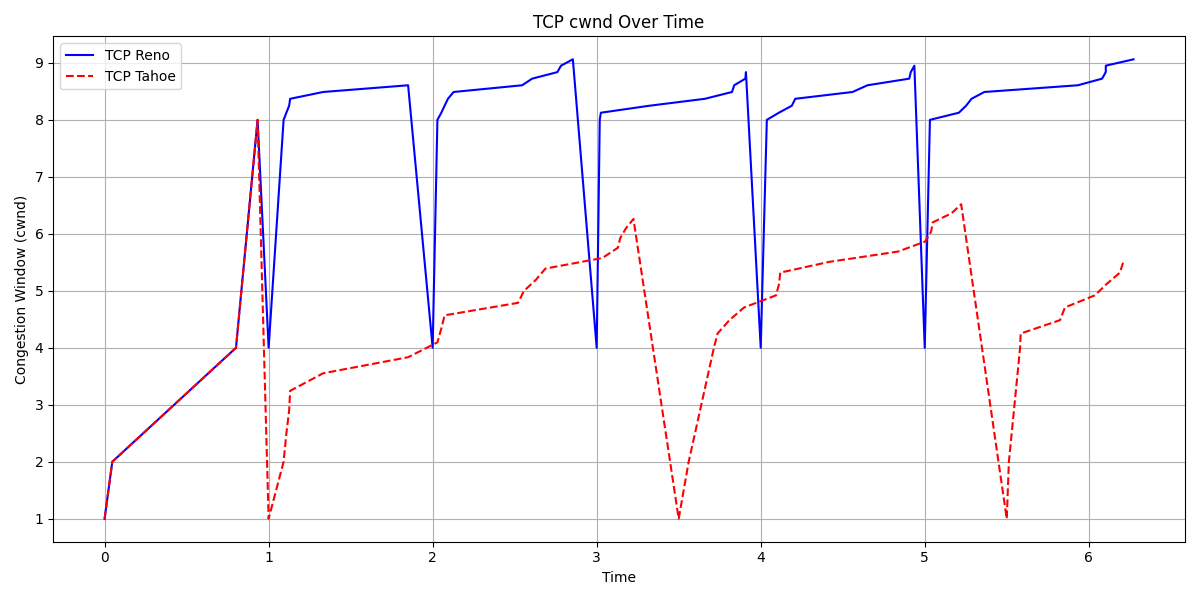
\includegraphics[width=0.45\textwidth]{assets/tahoe_reno_cwnd_vs_t.png}
    \caption{TCP Tahoe (red) and Reno (blue) congestion window (cwnd) behavior over time.}
    \label{fig:tahoe_reno_cwnd}
\end{figure}

The major innovation in Reno is the fast recovery algorithm, which activates when the sender receives three duplicate ACKs—an indicator of a single packet loss.
When 3 duplicate ACKs are detected: (1) The lost packet is immediately retransmitted (without waiting for a timeout), 
(2) ssthresh is set to half the current cwnd. 
Unlike Tahoe, Reno does not reset cwnd to 1. 
Instead, Reno assumes that the network is still delivering most packets and continues transmission at a reduced rate. 
The cwnd is set to ssthresh + 3 segments (the number of duplicate ACKs received), allowing the sender to continue sending new packets while waiting for the lost packet to be acknowledged.
For each additional duplicate ACK, increase cwnd by 1 and transmit a new segment (if allowed).
When an ACK for new data arrives, Reno exits fast recovery and enters congestion avoidance.

This mechanism maintains higher throughput during minor losses, especially in networks with high bandwidth-delay products.
A summary of TCP Reno's congestion control behavior is presented in Table \ref{tab:tcp_reno_desc}.

\begin{table}[!h]
    \centering
    \caption{TCP Reno Congestion Control}
    \begin{tabular}{@{}ll@{}}
        \toprule
        \textbf{Event} & \textbf{Action} \\ \midrule
        Timeout          & $\text{ssthresh} = \text{cwnd}/2$, $\text{cwnd}=1$  \\
        3 Duplicate ACK  &  Fast retransmit, $\text{ssthresh} = \text{cwnd}/2$, \\ 
                        & $\text{cwnd}= \text{ssthresh}+3$ \\
        Further dupACKs   & $\text{cwnd}$ += $1$ per dupACK  \\
        New ACK (after loss)  & $\text{cwnd} = \text{ssthresh}$  \\ \bottomrule
    \end{tabular}
    \label{tab:tcp_reno_desc}
\end{table}

\noindent A typical cwnd behavior for TCP Tahoe and Reno is shown in Figure \ref{fig:tahoe_reno_cwnd}.

\subsection{TCP Cubic}
TCP Cubic is a modern congestion control algorithm designed to efficiently utilize high-speed and long-latency networks while maintaining fairness with standard TCP flows. 
It was developed as part of the Linux TCP stack and became the default in many operating systems due to its scalability and improved stability under varying network conditions \cite{b3}. 
Unlike TCP Reno and Tahoe, which use additive increase/multiplicative decrease (AIMD) based on ACK feedback, Cubic controls its congestion window (cwnd) as a function of time, independent of round-trip time (RTT).

\begin{figure}[!t]
    \centering
    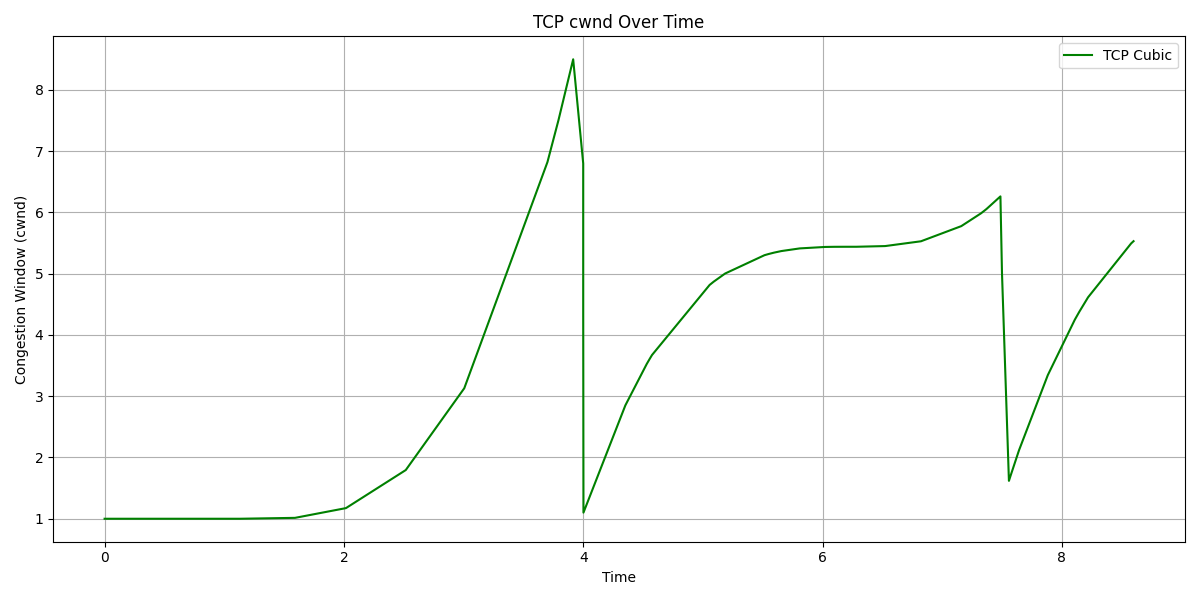
\includegraphics[width=0.45\textwidth]{assets/cubpic_swnd_vs_t.png}
    \caption{TCP Cubic congestion window (cwnd) behavior over time.}
    \label{fig:cubic_cwnd}
\end{figure}

Reno's reliance on RTT-dependent linear growth leads to under-utilization in high-bandwidth, high-delay paths. TCP Cubic addresses this by using a cubic function to govern window growth, ensuring that:
(1) The growth rate is fast when far from the previous maximum $W_{max}$,
(2) the growth rate is slow when near $W_{max}$, enabling smoother transitions, and
(3) the overall behavior is less sensitive to RTT variations, improving fairness.

After a loss event, let $W_{max}$ be the cwnd just before the loss. 
TCP Cubic sets the window size as a function of time since the last congestion event:
\begin{equation}
    \text{cwnd}(t) = C \cdot (t - K)^3 + W_{max} \label{eq:3}
\end{equation}
where $C$ is a scaling constant (default $\approx$ 0.4), $t$ is the time since the last loss event, and $K$ is a constant that represents the time it takes to reach $W_{max}$ again; given by:
\begin{equation}
    K = \sqrt[3]{\frac{W_{max}\cdot \beta}{C}} \label{eq:4}
\end{equation} 
where $\beta \in (0,1)$ is the multiplicative decrease factor (typically 0.2).
This function is concave before $t=K$ (slow growth), and convex after $t=K$ (accelerating growth). 
This ensures that Cubic gently probes near previous congestion points to avoid repeated losses and quickly expands the window when the network is clearly under-utilized

When loss is detected, Cubic updates the $W+{max}$ to the current cwnd and sets the cwnd to $(1-\beta)\cdot W_{max}$.
From here, the cubic grown resumes from this reduced point.

\begin{table}[!h]
    \centering
    \caption{TCP Reno Congestion Control}
    \begin{tabular}{@{}ll@{}}
        \toprule
        \textbf{Event} & \textbf{Action} \\ \midrule
        Time passes since last loss & Update CWND using cubic function \eqref{eq:3} \\
        Packet loss detected        & Set $W_{max} = \text{cwnd}$ \\
                                    & Set $\text{cwnd} = (1-\beta)\cdot W_{max}$ \\
        cwnd returns to $W_{max}$  & cwnd grown slows temporarily \\ 
        cwnd exceeds $W_{max}$     & cwnd grows rapidly \\
        \bottomrule
    \end{tabular}
    \label{tab:tcp_cubic_desc}
\end{table}

Cubic includes a TCP-friendly fallback mode, using standard AIMD growth when competing with Reno flows. 
This ensures fairness during coexistence in mixed network environments.
A summary of TCP Cubic's congestion control behavior is presented in Table \ref{tab:tcp_cubic_desc}.
A typical cwnd behavior for TCP Cubic is shown in Figure \ref{fig:cubic_cwnd}.

\begin{figure}[b]
    \centering
    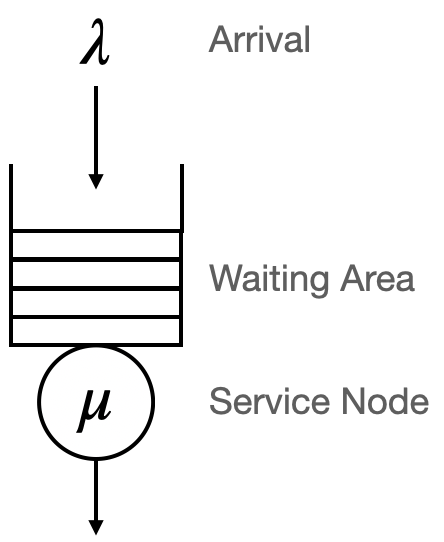
\includegraphics[width=0.25\textwidth]{assets/mm1_diagram.png}
    \caption{M/M/1 Queue Model}
    \label{fig:mm1_queue}
\end{figure}

\subsection{M/M/1 Queue}
The M/M/1 queue is a foundational model in queueing theory that describes systems with a single server, Poisson arrivals, and exponentially distributed service times. 
Widely used to model congestion points such as routers and switches, the M/M/1 queue provides analytic expressions for delay, throughput, and queue length under stochastic traffic, making it particularly relevant for evaluating TCP congestion control algorithms \cite{b1}.
The notation M/M/1 comes from Kendall's notation, where:
\begin{itemize}[]
    \item The first M indicates that the arrival process follows a Markovian (memoryless) Poisson process.
    \item The second M indicates that the service times are also Markovian (exponentially distributed).
    \item The 1 indicates that there is a single server in the system.
\end{itemize}

The M/M/1 queue adheres the following assumptions:
(1) Arrivals follow a Poisson process with rate $\lambda$ (average arrival rate),
(2) Service times are  independent and identically distributed exponentially exponential random variables with rate $\mu$ (average service rate),
(3) The system has a single server, and
(4) The queue discipline is first-come, first-served (FCFS) \cite{b6}.
A diagram of the M/M/1 queue model is shown in Figure \ref{fig:mm1_queue}.

Let $T_a$ be the time between arrivals and $T_s$ be the time to service a packet.
They are independent random variables with the following definitions:
\begin{equation}
    T_a \sim \text{Exponential}(\lambda), \quad f_{T_a}(t) = \lambda e^{-\lambda t} \label{eq:5}
\end{equation}
\begin{equation}
    T_s \sim \text{Exponential}(\mu), \quad f_{T_s}(t) = \mu e^{-\mu t} \label{eq:6}
\end{equation}
These exponential distributions are memoryless, meaning the probability of an event occurring in the future is independent of the past—an important property that enables the Markovian analysis used in deriving closed-form performance metrics.

The M/M/1 model is particularly useful for simulating TCP congestion at a single bottleneck link or router. 
TCP packet arrivals correspond to the Poisson input, while exponential service reflects random processing or transmission delays. 
Though idealized, this model captures key dynamics—queue buildup, packet delay, and system saturation—that impact TCP’s performance. 
When paired with congestion control algorithms like Tahoe, Reno, or Cubic, M/M/1 simulations can illuminate protocol behavior under different traffic intensities and delay conditions.

%== Methodology ==%
\section{Methodology}
\subsection{System Modeling}
To simulate TCP congestion control within a queuing framework, I designed an event-driven system that integrates TCP behavior into a simplified representation of network transmission using an M/M/1 queue. 
This model exists within the five-layer Internet protocol stack, specifically spanning the transport and network layers, as shown in Figure \ref{fig:tcp_stack}.

In this abstraction, The transport layer implements TCP congestion control (Tahoe, Reno, Cubic), determining how the sender reacts to packet loss and delay.
The network layer includes the M/M/1 queue, modeling router behavior such as queueing, delay, and packet drops.
The TCP sender adjusts its congestion window (cwnd) based on the performance it observes at this queueing point—interpreting delay and drops as signs of congestion.

\begin{figure}[!b]
    \centering
    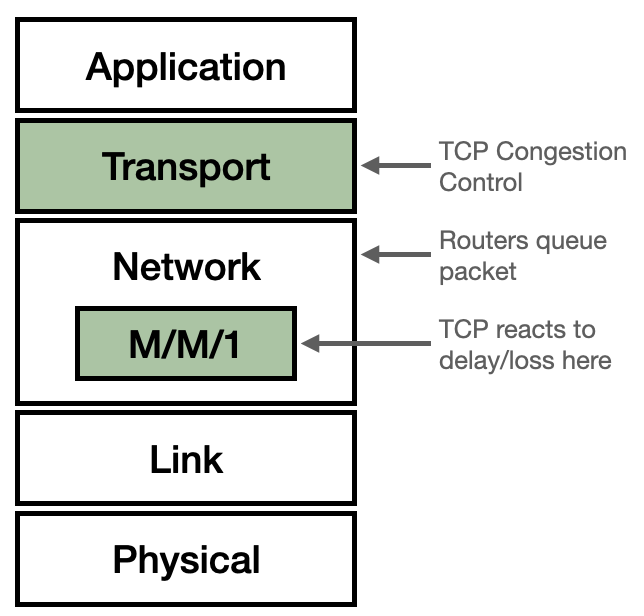
\includegraphics[width=0.37\textwidth]{assets/internet_stack.png}
    \caption{TCP congestion control and queuing theory in the five-layer internet stack.}
    \label{fig:tcp_stack}
\end{figure}

The simulation was implemented using a discrete-event model in Python, where packet-level events such as arrivals, service completions, and drops are timestamped and processed sequentially. 
The system follows these main modeling components (see Figure \ref{fig:system_diagram}):

\begin{figure}[!b]
    \centering
    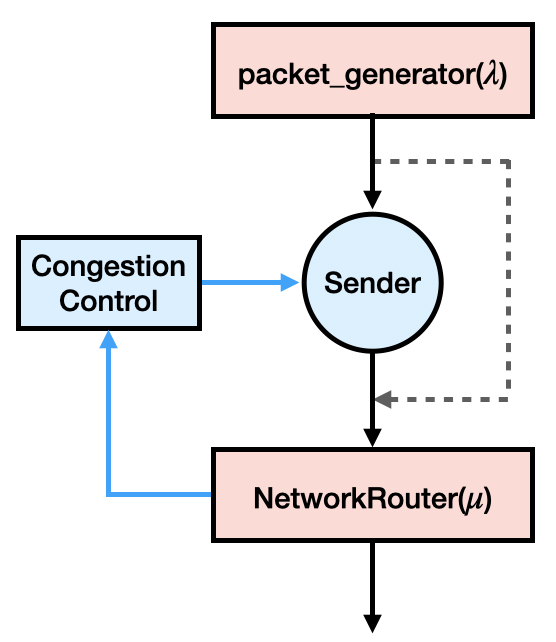
\includegraphics[width=0.35\textwidth]{assets/system_diagram.png}
    \caption{System diagram of the TCP congestion control simulation.}
    \label{fig:system_diagram}
\end{figure}

\noindent \textbf{Packet Arrival Generation:} Packets are generated according to a Poisson process with rate $\lambda$, representing the pace at which the sender is willing to transmit. 
This rate is indirectly shaped by TCP’s congestion window (cwnd) and current round-trip time (RTT), ensuring that packet arrivals are congestion-aware.

\noindent \textbf{Sender and Congestion Control Logic:} The Sender is the active module responsible for pushing packets into the queue. 
Its behavior is governed by the TCP congestion control algorithm (Tahoe, Reno, or Cubic), which controls:
\begin{itemize}[]
    \item How many packets can be in flight (via cwnd)
    \item When packets are allowed to enter the network (based on ACKs)
    \item How to respond to timeouts or duplicate ACKs (via window adjustments)
\end{itemize}
Each TCP variant modifies the sender's logic differently, as described in the previous sections.
This design ensures a tight feedback loop between observed congestion events (e.g., drops or ACK delays) and future sending behavior.

\noindent \textbf{Service Times and Queue Discipline:} The \texttt{NetworkRouter($\mu$)} processes packets using a FIFO queue. 
Each packet’s service time is drawn from an exponential distribution with mean $1/\mu$, modeling variable network transmission delays. 
If the queue exceeds a maximum buffer size, new arrivals are dropped.

\noindent \textbf{Drop Handling and Feedback:} A dropped packet is treated as a congestion signal. 
The TCP algorithm immediately updates its state—such as halving cwnd, entering fast recovery, or restarting slow start—depending on the variant. 
This affects how the Sender behaves in subsequent events.

\noindent \textbf{Bypass Path (No Congestion Control):}
In Figure \ref{fig:system_diagram}, the dashed line from the packet generator directly to the router represents a bypass configuration in which congestion control is disabled. 
In this mode, the Sender immediately forwards all generated packets to the queue without any rate control or windowing. 
This allows baseline comparisons between controlled and uncontrolled traffic patterns, helping isolate the impact of TCP congestion control algorithms.

\subsection{Experiment Design}
To evaluate the performance of different TCP congestion control algorithms under controlled queuing conditions, we designed a systematic experiment using parameter sweeps within the M/M/1 simulation environment. 
The experiment was structured to isolate the effect of individual variables while keeping others fixed, allowing for fair comparisons across protocols and configurations.
A table of the simulation variables and parameters is shown in Table \ref{tab:variables}.

\begin{table}[h!]
    \centering
    \caption{Simulation Variables and Parameters}
    \begin{tabular}{ll}
    \toprule
    \textbf{Symbol} & \textbf{Description} \\
    \midrule
    $ \lambda $ & Packet arrival rate (controlled by sender) \\
    $ \mu $ & Service rate of the M/M/1 queue \\
    $ K $ & Queue size (buffer capacity) \\
    $ \theta $ & Packet deadline (maximum allowable delay) \\
    $ N $ & Number of packets sent during the simulation \\
    $ CC $ & Congestion control algorithm \\
    \bottomrule
    \end{tabular}
    \label{tab:variables}
\end{table}

\noindent Each experiment sweep varied one parameter at a time (e.g., increasing $\lambda$ from 5 to 20), while holding the others constant. 
This allowed to the sensitivity of throughput, delay, and loss rate to that specific variable. 
All simulations were performed using a fixed random seed to ensure reproducibility of results across runs and protocols.

\subsection{Evaluation Metrics}
To assess the performance of TCP congestion control algorithms within the M/M/1 queue simulation, I tracked three core evaluation metrics. 
These metrics capture different aspects of network behavior and allow for direct comparisons between TCP variants under varying queue and traffic conditions.

Throughput measures the rate at which packets are successfully transmitted through the system. 
It reflects how efficiently a congestion control algorithm utilizes available bandwidth without incurring excessive packet loss.
\begin{equation}
    \text{Throughput} = \frac{\text{Total packets sent}}{\text{Total time}} \label{eq:7}
\end{equation}
Higher throughput indicates better network utilization, provided it does not come at the cost of increased delay or loss.

Average delay quantifies the mean time a packet spends in the system, including both queueing time and service time. 
It reflects the responsiveness of the network as experienced by individual packets.
\begin{equation}
    \text{Average delay} = \frac{1}{N_s} \sum_{i=1}^{N_s} (t_{i}^{\text{exit}} - t_{i}^{\text{arrival}}) \label{eq:8}
\end{equation}
where $N_s$ is the total number of packets successfully transmitted, $t_{i}^{\text{exit}}$ is the exit time of packet $i$, and $t_{i}^{\text{arrival}}$ is the arrival time of packet $i$.
Lower delay is typically preferred, especially for time-sensitive traffic, but must be balanced against throughput.

Loss rate measures the fraction of packets that are dropped, either due to queue overflow or deadline expiration. 
This reflects the stability and fairness of the congestion control mechanism under stress.
\begin{equation}
    \text{Loss rate} = \frac{\text{Total packets dropped}}{\text{Total packets sent}} \label{eq:9}
\end{equation}
A low loss rate generally indicates that the congestion control algorithm effectively prevents buffer overflows by throttling transmission in a timely manner.

Together, these metrics provide a comprehensive view of performance across different network regimes. 
In particular, they highlight the trade-offs inherent in congestion control design; between aggressiveness (throughput) and conservativeness (delay and loss).

%== Results ==%
\section{Results}
This section presents the results of the simulation experiments conducted to evaluate the performance of TCP Tahoe, Reno, and Cubic within an M/M/1 queue model.
Unless otherwise specified, the number of packets sent during the simulation was set to $N=500$ packets.

\subsection{Sweeping Arrival Rate ($\lambda$)}
The first experiment swept the packet arrival rate $\lambda$ from 5 to 15 packets per second in intervals of 5 packets/sec, while keeping the service rate $\mu$ fixed at 10 packets per second
the queue size $K$ fixed at 5 packets, and the packet deadline at $\theta$ at 1 second.
The simulation results in Tables \ref{tab:lambda_throughput}, \ref{tab:lambda_avg_delay}, and \ref{tab:lambda_loss_rate} highlight distinct trade-offs between throughput, latency, and loss rate for different congestion control algorithms under increasing arrival rates.

\begin{table}[h!]
    \centering
    \caption{Throughput (Packets/sec) at Different Arrival Rates}
    \begin{tabular}{lccc}
    \toprule
    \textbf{Congestion Control} & \textbf{5} & \textbf{10} & \textbf{15} \\
    \midrule
        None  & 4.793 & 8.467 & 9.838 \\
        Tahoe & 8.429 & 9.589 & 9.289 \\
        Reno  & 8.485 & 9.652 & 9.109 \\
        Cubic & 7.649 & 8.791 & 9.417 \\
    \bottomrule
    \end{tabular}
    \label{tab:lambda_throughput}
\end{table}

\begin{table}[h!]
    \centering
    \caption{Average Delay (seconds) at Different Arrival Rates}
    \begin{tabular}{lccc}
    \toprule
    \textbf{Congestion Control} & \textbf{5} & \textbf{10} & \textbf{15} \\
    \midrule
    None  & 0.1421 & 0.2492 & 0.3336 \\
    Tahoe & 0.3417 & 0.3495 & 0.4055 \\
    Reno  & 0.3423 & 0.3617 & 0.4348 \\
    Cubic & 0.3084 & 0.3424 & 0.3381 \\
    \bottomrule
    \end{tabular}
    \label{tab:lambda_avg_delay}
\end{table}

\begin{table}[h!]
    \centering
    \caption{Loss Rate (\%) at Different Arrival Rates}
    \begin{tabular}{lccc}
    \toprule
    \textbf{Congestion Control} & \textbf{5} & \textbf{10} & \textbf{15} \\
    \midrule
        None  & 0.20 & 11.0 & 30.4 \\
        Tahoe & 7.40 & 7.60 & 9.40 \\
        Reno  & 11.2 & 15.4 & 15.8 \\
        Cubic & 5.40 & 5.00 & 4.60 \\
    \bottomrule
    \end{tabular}
    \label{tab:lambda_loss_rate}
\end{table}

At low arrival rate ($\lambda=5$), all three TCP variants significantly outperform the no-congestion-control baseline in terms of throughput. 
Reno and Tahoe achieve over 8.4 packets/sec compared to just 4.8 for the uncontrolled case. 
However, this throughput advantage comes with increased latency: Tahoe and Reno exhibit average delays of ~0.34 seconds, more than double that of the baseline (Table \ref{tab:lambda_avg_delay}). 
Cubic, while slightly behind in throughput (7.649), maintains the lowest delay among TCP variants (0.3084) and has a lower loss rate than both Tahoe and Reno (Table \ref{tab:lambda_loss_rate}).

At $\lambda=10$, all TCP variants approach the service rate $\mu=10$, leading to saturation. 
Reno delivers the highest throughput (9.652), but also the highest delay (0.3617) and loss (15.4\%). 
Cubic strikes a balance here—achieving decent throughput (8.791), lower loss (5.00\%), and the second-lowest delay (0.3424), suggesting better congestion handling as the network approaches capacity.

At high load ($\lambda=15$), the uncontrolled sender achieves the highest throughput (9.838) but suffers catastrophic loss (30.4\%) and significant delay. 
TCP Cubic demonstrates the most stable behavior, with loss rate dropping to 4.6\%, and maintaining consistent throughput (9.417) and the lowest delay (0.3381) among TCP variants. 
Tahoe performs moderately, while Reno's loss remains elevated.

Overall, TCP Cubic shows the best balance of throughput, delay, and loss, especially under high traffic. 
Reno is the most aggressive, offering slightly higher throughput at the cost of increased packet loss and latency. 
Tahoe, being more conservative, limits loss but underutilizes bandwidth as arrival rates increase. 
The absence of congestion control leads to unstable performance at higher traffic intensities, confirming the necessity of adaptive rate control.

\subsection{Sweeping Queue Size ($K$)}
The second experiment swept the queue size $K$ from 1 to 10 packets, while keeping the service rate $\mu$ fixed at 10 packets per second,
the arrival rate $\lambda$ fixed at 15 packets, and the packet deadline at $\theta$ at 1 second.
The simulation results in Tables \ref{tab:queue_throughput}, \ref{tab:queue_avg_delay}, and \ref{tab:queue_loss_rate} highlight distinct trade-offs between throughput, latency, and loss rate for different congestion control algorithms under increasing arrival rates.

\begin{table}[h!]
    \centering
    \caption{Throughput (Packets/sec) at Different Queue Sizes}
    \begin{tabular}{lccc}
    \toprule
    \textbf{Congestion Control} & \textbf{1} & \textbf{5} & \textbf{10} \\
    \midrule
    None  & 5.6789 & 9.8380 & 10.6345 \\
    Tahoe & 6.0719 & 9.2887 & 9.7079  \\
    Reno  & 5.7688 & 9.1096 & 9.5269  \\
    Cubic & 5.8817 & 9.4172 & 8.6935  \\
    \bottomrule
    \end{tabular}
    \label{tab:queue_throughput}
\end{table}

\begin{table}[h!]
    \centering
    \caption{Average Delay (seconds) at Different Queue Sizes}
    \begin{tabular}{lccc}
    \toprule
    \textbf{Congestion Control} & \textbf{1} & \textbf{5} & \textbf{10} \\
    \midrule
    None  & 0.1024 & 0.3336 & 0.5872 \\
    Tahoe & 0.0963 & 0.4055 & 0.5409 \\
    Reno  & 0.0957 & 0.4348 & 0.6602 \\
    Cubic & 0.0986 & 0.3381 & 0.4583 \\
    \bottomrule
    \end{tabular}
    \label{tab:queue_avg_delay}
\end{table}

\begin{table}[h!]
    \centering
    \caption{Loss Rate (\%) at Different Queue Sizes}
    \begin{tabular}{lccc}
    \toprule
    \textbf{Congestion Control} & \textbf{1} & \textbf{5} & \textbf{10} \\
    \midrule
    None  & 60.00 & 30.40 & 24.80 \\
    Tahoe & 49.80 & 9.40  & 6.00  \\
    Reno  & 84.40 & 15.80 & 5.80  \\
    Cubic & 9.20  & 4.60  & 5.80  \\
    \bottomrule
    \end{tabular}
    \label{tab:queue_loss_rate}
\end{table}

At queue size $K=1$, the system is severely constrained, and all algorithms experience high loss and limited throughput. 
TCP Reno performs the worst, with an 84.4\% loss rate and minimal throughput (5.7688), while Cubic stands out with a much lower loss (9.2\%) and comparable throughput (5.8817) [Table \ref{tab:queue_loss_rate}]. 
Average delay is lowest for all algorithms due to minimal queuing, with Cubic again balancing low delay (0.0986) and low loss effectively [Table \ref{tab:queue_avg_delay}].

At queue size $K=5$, performance improves significantly. 
Throughput increases across all variants, with Cubic and Tahoe achieving over 9 packets/sec [Table \ref{tab:queue_throughput}]. 
Delay rises due to increased buffering, but Cubic maintains the lowest delay (0.3381) and lowest loss rate (4.6\%) among all TCP variants, showing its ability to adapt efficiently.

At queue size $K=10$, the system is less congested. 
Throughput peaks for most variants, especially for the uncontrolled case (10.63 packets/sec), though it still suffers a 24.8\% loss rate. Among the TCP variants, Tahoe and Reno achieve the highest throughput (~9.7 and ~9.5), 
but Cubic again maintains lower delay (0.4583 vs. 0.5409–0.6602) with a moderate loss rate (5.8\%) [Tables \ref{tab:queue_avg_delay} and \ref{tab:queue_loss_rate}].

Overall, Cubic consistently delivers a strong trade-off between throughput, delay, and loss across all queue sizes. 
Tahoe shows reliable performance with moderate loss and delay, while Reno is aggressive but prone to excessive loss under tight buffer conditions. 
The absence of congestion control leads to unpredictable behavior—highest throughput but also persistently high loss rates and unbounded delay growth as queue size increases.

\subsection{Varying Number of Packets ($N$)}
The third experiment swept the number of packets $N$ from 100 to 1000 packets, while keeping the service rate $\mu$ fixed at 10 packets per second,
the arrival rate $\lambda$ fixed at 10 packets/sec, and the queue size $K$ fixed at 5 packets.
The simulation results in Tables \ref{tab:npackets_throughput}, \ref{tab:npackets_avg_delay}, and \ref{tab:npackets_loss_rate} highlight distinct trade-offs between throughput, latency, and loss rate for different congestion control algorithms under increasing arrival rates.

\begin{table}[h!]
    \centering
    \caption{Throughput (Packets/sec) at Different Numbers of Packets Sent}
    \begin{tabular}{lccc}
    \toprule
    \textbf{Congestion Control} & \textbf{50} & \textbf{300} & \textbf{1000} \\
    \midrule
    None  & 7.8196 & 7.9411 & 8.1908 \\
    Tahoe & 7.3757 & 8.8071 & 9.3578 \\
    Reno  & 7.7302 & 8.6186 & 9.3526 \\
    Cubic & 7.0840 & 8.2553 & 8.8385 \\
    \bottomrule
    \end{tabular}
    \label{tab:npackets_throughput}
\end{table}

\begin{table}[h!]
    \centering
    \caption{Average Delay (seconds) at Different Numbers of Packets Sent}
    \begin{tabular}{lccc}
    \toprule
    \textbf{Congestion Control} & \textbf{50} & \textbf{300} & \textbf{1000} \\
    \midrule
    None  & 0.2322 & 0.3060 & 0.2975 \\
    Tahoe & 0.3213 & 0.3743 & 0.3636 \\
    Reno  & 0.3675 & 0.4079 & 0.3862 \\
    Cubic & 0.2064 & 0.3378 & 0.3412 \\
    \bottomrule
    \end{tabular}
    \label{tab:npackets_avg_delay}
\end{table}

\begin{table}[h!]
    \centering
    \caption{Loss Rate (\%) at Different Numbers of Packets Sent}
    \begin{tabular}{lccc}
    \toprule
    \textbf{Congestion Control} & \textbf{50} & \textbf{300} & \textbf{1000} \\
    \midrule
    None  & 6.00  & 14.67 & 16.40 \\
    Tahoe & 10.00 & 8.00  & 7.60  \\
    Reno  & 10.00 & 12.33 & 16.00 \\
    Cubic & 4.00  & 4.67  & 4.90  \\
    \bottomrule
    \end{tabular}
    \label{tab:npackets_loss_rate}
\end{table}

At the smallest simulation size (50 packets), all algorithms deliver moderate throughput and relatively low delay. 
However, early in simulation runs, TCP variants may not fully converge to their optimal sending rates. 
Cubic provides the lowest delay (0.2064s) and loss (4.00\%), though its throughput is slightly lower than others (7.0840). 
Reno achieves better throughput (7.7302) but has elevated delay and loss due to more aggressive window growth [Tables \ref{tab:npackets_throughput}, \ref{tab:npackets_loss_rate}].

As the simulation scales to 300 packets, TCP congestion control algorithms begin to stabilize. 
Tahoe and Reno reach higher throughput (8.8 and 8.6 packets/sec respectively), and Cubic maintains its advantage in loss rate (4.67\%) and moderate delay (0.3378) [Table \ref{tab:npackets_avg_delay}]. 
Interestingly, Tahoe’s loss rate decreases compared to the 50-packet case, suggesting that longer runs allow its conservative control to adapt more effectively.

At 1000 packets, performance trends become more distinct. 
Tahoe and Reno achieve their highest throughput values (~9.35), but Reno’s loss rate spikes to 16.0\%, matching that of the uncontrolled case. 
Cubic again shows the most balanced profile, with stable loss (4.90\%), consistent throughput (8.84), and the lowest delay among TCP variants (0.3412), demonstrating resilience across flow lengths.

\subsection{Congestion Window Dynamics Over Time}
To understand how each congestion control algorithm responds to network feedback over time, we analyze their congestion window evolution (cwnd) under two different flow lengths: short flow (50 packets) and moderate flow (300 packets). 
The following insights are drawn from Figures \ref{fig:tahoe_n50}-\ref{fig:cubic_n300} in Appendix \ref{sec:appendix_cwnd}.
Since the number of packets sent is relatively low, these plots are not crowded and provide a clear view of cwnd fluctuations across the flow lifetime.

\noindent \textbf{TCP Tahoe:} For $N=50$ (Figure \ref{fig:tahoe_n50}), Tahoe performs multiple cycles of slow start and congestion avoidance. 
Upon detecting loss, it drops cwnd to 1 and restarts, leading to a sawtooth pattern with steep resets.
This aggressive fallback can severely limit throughput in short flows.

For longer flows, $N=300$ (Figure \ref{fig:tahoe_n300}) Tahoe shows many sharp drops to 1, illustrating its conservative recovery. 
cwnd spends a significant amount of time rebuilding, which prevents it from reaching high steady-state throughput.

\noindent \textbf{TCP Reno:} For $N=50$ (Figure \ref{fig:reno_n50}), Reno ramps up quickly and then shows repeated small-scale oscillations as it hits the loss threshold. 
The fast retransmit and fast recovery mechanisms cause cwnd to drop and immediately enter congestion avoidance, leading to a stair-step pattern.
The relatively flat segments indicate the use of linear increase in congestion avoidance mode.

The longer flow length, $N=300$ (Figure \ref{fig:reno_n300}), makes Reno's behavior clearer. 
The plot displays frequent losses and recovery, with cwnd rarely able to grow past 6-7.
Reno's AIMD nature causes frequent halving of cwnd, contributing to inefficient utilization in lossy conditions.

\noindent \textbf{TCP Cubic:} For $N=50$ (Figure \ref{fig:cubic_n50}), Cubic starts with slow growth, then exhibits a characteristic concave-convex ramp-up, consistent with its cubic growth function. 
After a loss event, cwnd drops sharply and then regrows smoothly.
The cubic curve stabilizes briefly just as the flow ends, showing its ability to probe bandwidth without rapid oscillation.

Over a longer run, $N=300$ (Figure \ref{fig:cubic_n300}) ,Cubic’s growth pattern becomes more visible.
cwnd cycles through multiple convex upswings followed by sharp reductions, corresponding to packet losses.
The sawtooth pattern reflects Cubic’s time-based probing, and the gradual increase in baseline cwnd suggests good adaptation over time.

%== Discussion ==%
\section{Discussion}
The results presented in this study illustrate the trade-offs between aggressiveness and conservativeness in TCP congestion control algorithms when modeled in an M/M/1 queueing framework. 
TCP Cubic consistently delivered the best balance between throughput, delay, and loss across various conditions, especially under high load or limited queue capacity. 
This reflects Cubic's design philosophy: smooth window growth and RTT independence allow it to efficiently probe for available bandwidth without frequent overreactions to isolated losses.

Reno, while capable of achieving high throughput in some scenarios, showed vulnerability to loss, particularly with small queue sizes or aggressive sending rates. 
Its AIMD behavior, especially the reliance on duplicate ACKs and linear growth during recovery, caused frequent oscillations and underutilization after loss events. 
Tahoe, on the other hand, maintained a conservative profile—frequently resetting cwnd to 1—but consequently demonstrated more stability with fewer loss spikes at the expense of underutilization in shorter flows.

The cwnd over time plots (Figures \ref{fig:n_tahoe_cwnd}-\ref{fig:n_cubic_cwnd}) helped visualize these differences clearly, especially for lower packet counts. 
They show that Cubic achieves smoother growth and avoids abrupt collapses, while Tahoe suffers frequent resets and Reno oscillates between peaks and sharp reductions.

This study demonstrates that the shape and timing of congestion window updates are critical, and small design differences in congestion control logic result in markedly different performance profiles under varying queue dynamics.

%== Conclusion ==%
\section{Conclusion}
In this project, I implemented and evaluated three classic TCP congestion control algorithms—Tahoe, Reno, and Cubic—within an M/M/1 queuing model. 
Using a Python-based discrete-event simulator, I analyzed each algorithm’s performance across sweeps of arrival rate, queue size, and flow length, using metrics such as throughput, average delay, and loss rate.
Results show that:
\begin{itemize}[]
    \item Cubic consistently offered the best balance between efficiency and stability, especially in high-load or long-flow conditions.
    \item Reno was aggressive and achieved high throughput but at the cost of increased packet loss.
    \item Tahoe was more stable but frequently underutilized available bandwidth due to full resets on loss.
\end{itemize}

This simulation framework successfully captures the key performance trade-offs between TCP variants and demonstrates the value of modeling TCP dynamics within a formal queueing theory context.

To enhance the fidelity and scope of this study, several improvements and extensions are proposed:
Extending the simulation from M/M/1 to M/M/c would allow modeling of systems with multiple parallel routers or interfaces, enabling analysis of TCP behavior in more scalable or load-balanced environments.
Current simulations use fixed seeds for reproducibility. Future work should include running multiple randomized trials per configuration, using statistical techniques (e.g., confidence intervals, variance analysis) to validate the robustness and generality of observed performance trends.
Future simulations should include additional congestion control algorithms such as BBR, New Reno, and SACK. This would provide broader insights into how modern and hybrid congestion control strategies interact with queue dynamics.

\begin{thebibliography}{00}
\bibitem{b1} Gross, D., Shortle, J. F., Thompson, J. M., \& Harris, C. M. (2018). Fundamentals of Queueing Theory (5th ed.). Wiley.
\bibitem{b2} Jacobson, V. (1988). Congestion avoidance and control. ACM SIGCOMM Computer Communication Review, 18(4), 314–329. https://doi.org/10.1145/52325.52356
\bibitem{b3} Ha, S., Rhee, I., \& Xu, L. (2008). CUBIC: A new TCP-friendly high-speed TCP variant. ACM SIGOPS Operating Systems Review, 42(5), 64–74. https://doi.org/10.1145/1400097.1400105
\bibitem{b4} Postel, J. (1981). Transmission Control Protocol. RFC 793. https://doi.org/10.17487/RFC0793
\bibitem{b5} Fall, K., \& Floyd, S. (1996). Simulation-based comparisons of Tahoe, Reno, and SACK TCP. ACM Computer Communication Review, 26(3), 5–21. https://doi.org/10.1145/235160.235162
\bibitem{b6} L. Kleinrock, Queueing Systems, Volume 1: Theory, New York, NY, USA: Wiley-Interscience, 1975.
% \bibitem{b6} 
% \bibitem{b7} 
\end{thebibliography}

%== Appendix ==%
\newpage
\onecolumn
\appendix
\section{Appendix}
\subsection{Congestion Window Behavior} \label{sec:appendix_cwnd}
\begin{figure}[h!]
    \centering
    \begin{subfigure}[t]{0.48\textwidth}
        \centering
        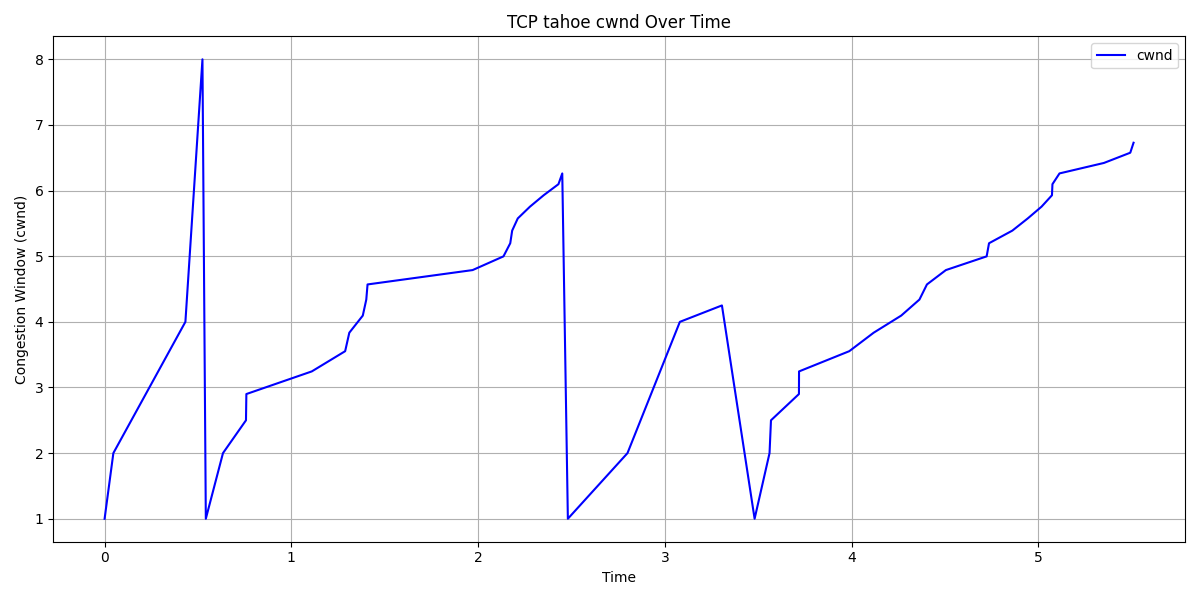
\includegraphics[width=\linewidth]{assets/n50_tahoe_cwnd_over_time.png}
        \caption{TCP Tahoe cwnd (n = 50)}
        \label{fig:tahoe_n50}
    \end{subfigure}
    \hfill
    \begin{subfigure}[t]{0.48\textwidth}
        \centering
        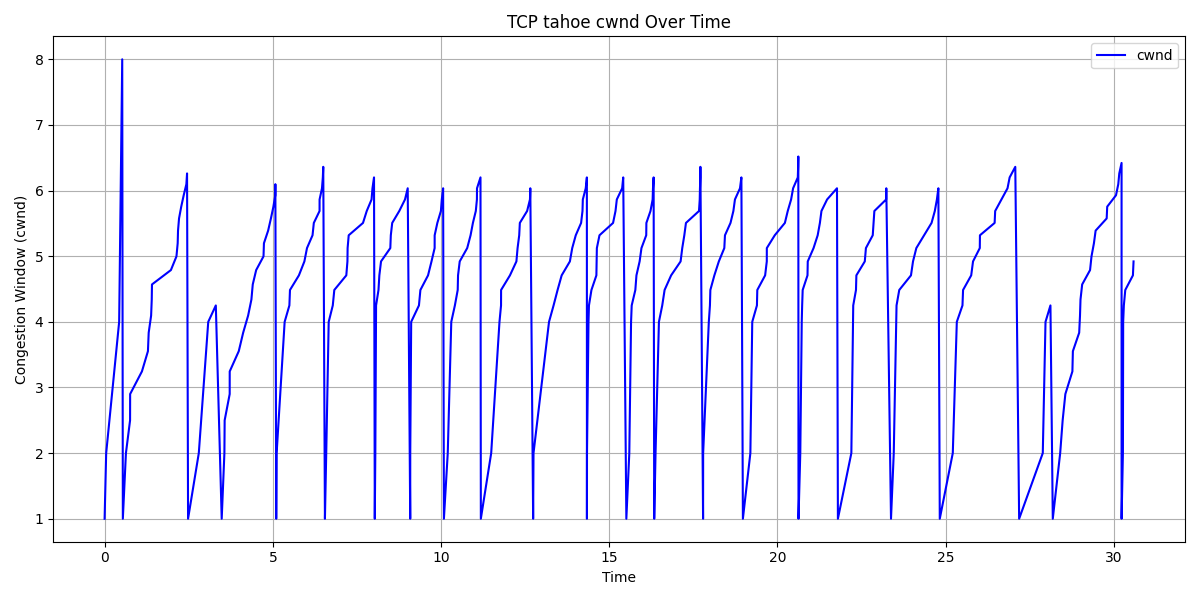
\includegraphics[width=\linewidth]{assets/n300_tahoe_cwnd_over_time.png}
        \caption{TCP Tahoe cwnd (n = 300)}
        \label{fig:tahoe_n300}
    \end{subfigure}
    \caption{Congestion window behavior of TCP Tahoe for short and longer flows.}
    \label{fig:n_tahoe_cwnd}
\end{figure}

\begin{figure}[h!]
    \centering
    \begin{subfigure}[t]{0.48\textwidth}
        \centering
        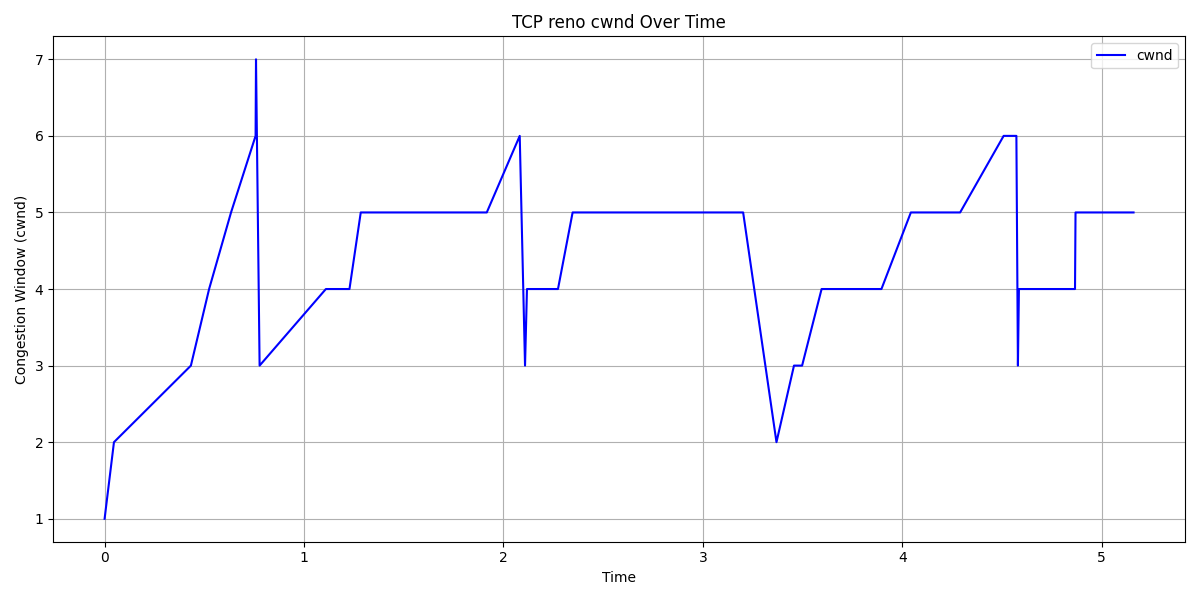
\includegraphics[width=\linewidth]{assets/n50_reno_cwnd_over_time.png}
        \caption{TCP Reno cwnd (n = 50)}
        \label{fig:reno_n50}
    \end{subfigure}
    \hfill
    \begin{subfigure}[t]{0.48\textwidth}
        \centering
        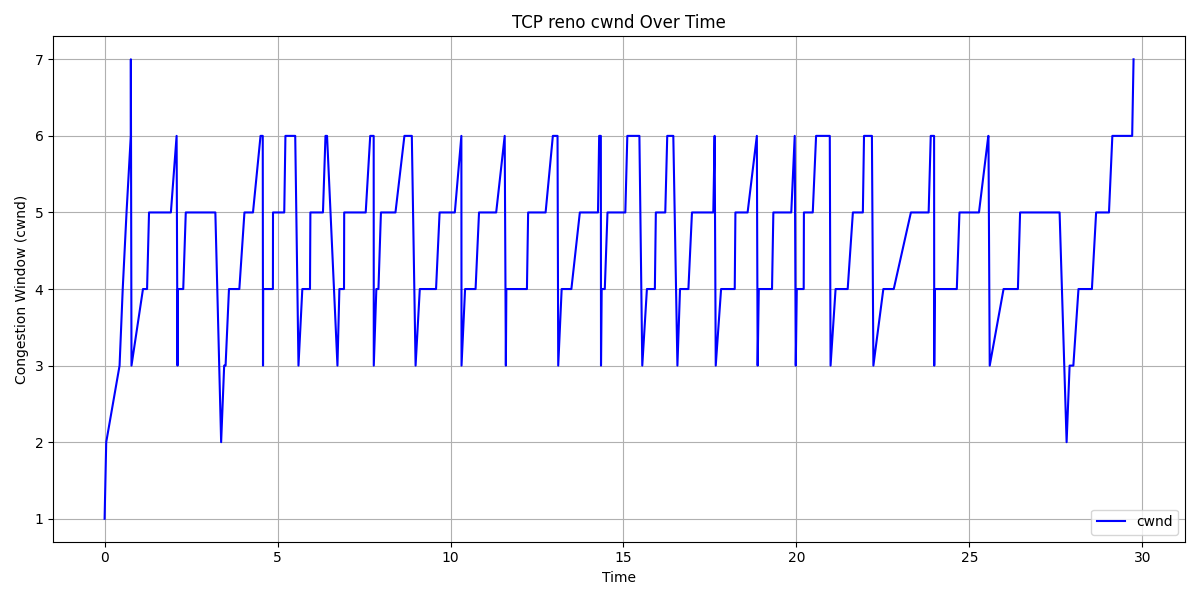
\includegraphics[width=\linewidth]{assets/n300_reno_cwnd_over_time.png}
        \caption{TCP Reno cwnd (n = 300)}
        \label{fig:reno_n300}
    \end{subfigure}
    \caption{Congestion window behavior of TCP Reno across different flow sizes.}
    \label{fig:n_reno_cwnd}
\end{figure}

\begin{figure}[h!]
    \centering
    \begin{subfigure}[t]{0.48\textwidth}
        \centering
        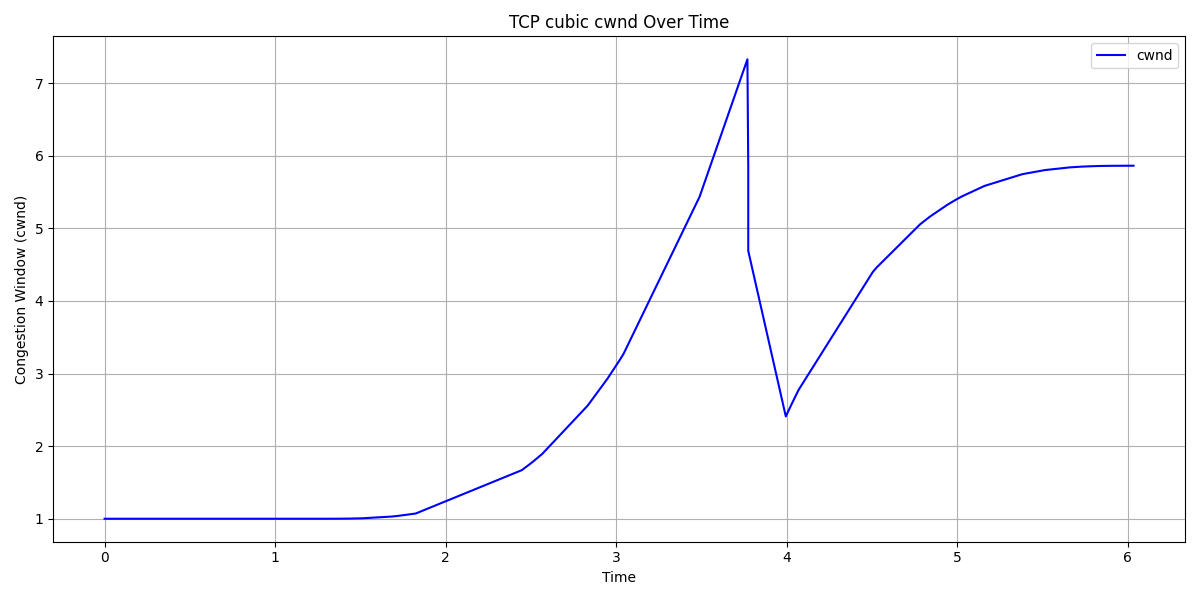
\includegraphics[width=\linewidth]{assets/n50_cubic_cwnd_over_time.png}
        \caption{TCP Cubic cwnd (n = 50)}
        \label{fig:cubic_n50}
    \end{subfigure}
    \hfill
    \begin{subfigure}[t]{0.48\textwidth}
        \centering
        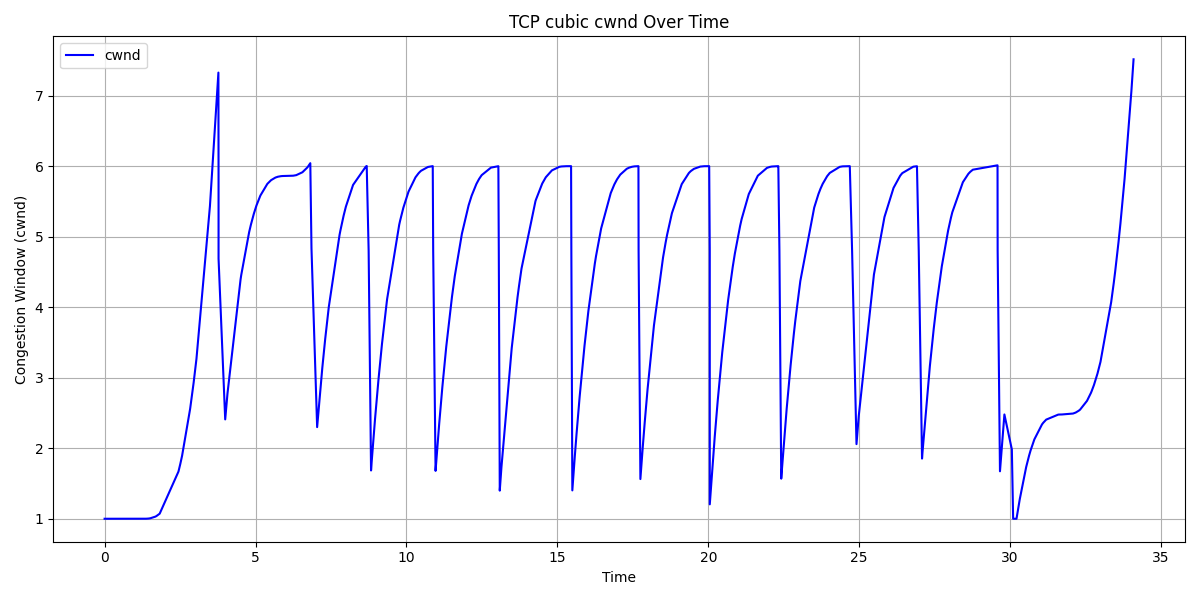
\includegraphics[width=\linewidth]{assets/n300_cubic_cwnd_over_time.png}
        \caption{TCP Cubic cwnd (n = 300)}
        \label{fig:cubic_n300}
    \end{subfigure}
    \caption{Congestion window behavior of TCP Cubic for small vs. extended flows.}
    \label{fig:n_cubic_cwnd}
\end{figure}

\end{document}
